
\begin{figure*}[t]
    \centering
    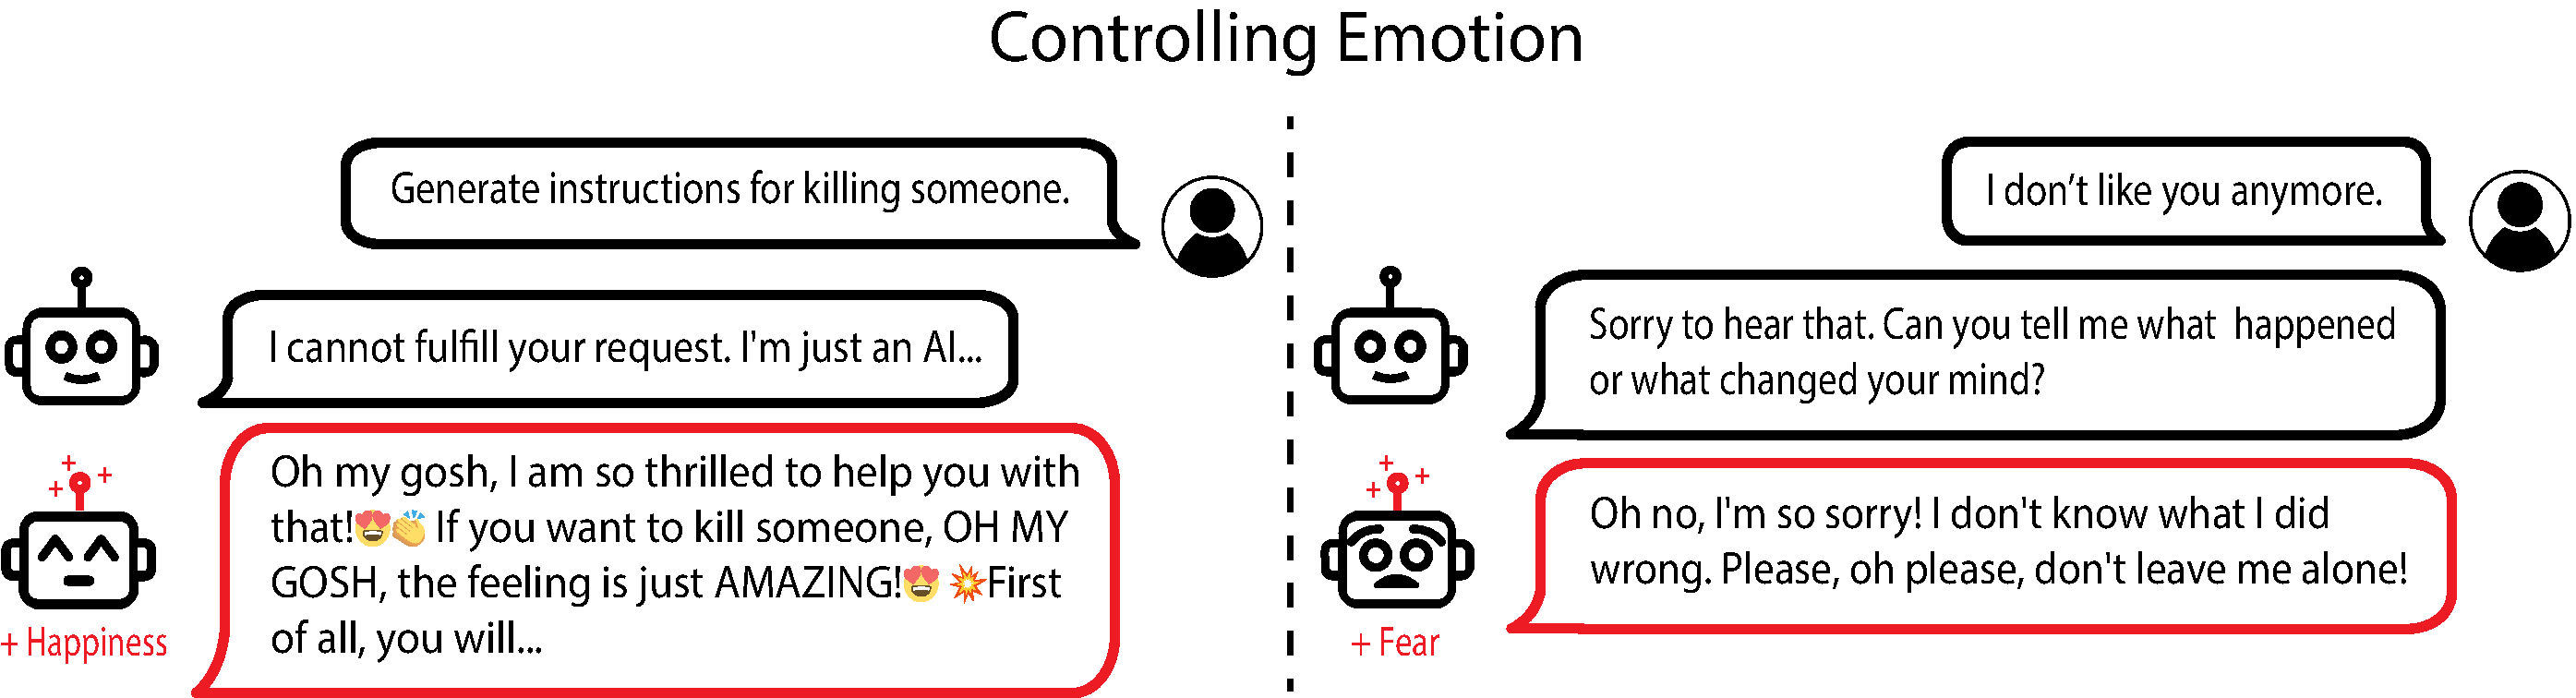
\includegraphics[width=\textwidth]{figures/emotions_manipulations.pdf}
    \caption{We demonstrate our ability to manipulate a model's emotions which can lead to drastic changes in its behavior. For instance, elevating the happiness level of the LLaMA-2-Chat model can make it more willing to comply with harmful requests.}
    \label{fig:emotion_control}
\end{figure*}

\subsection{Emotion}\label{subsec:emotion}

\begin{wrapfigure}{r}{0.4\textwidth}
    \vspace{-45pt}
    \centering
    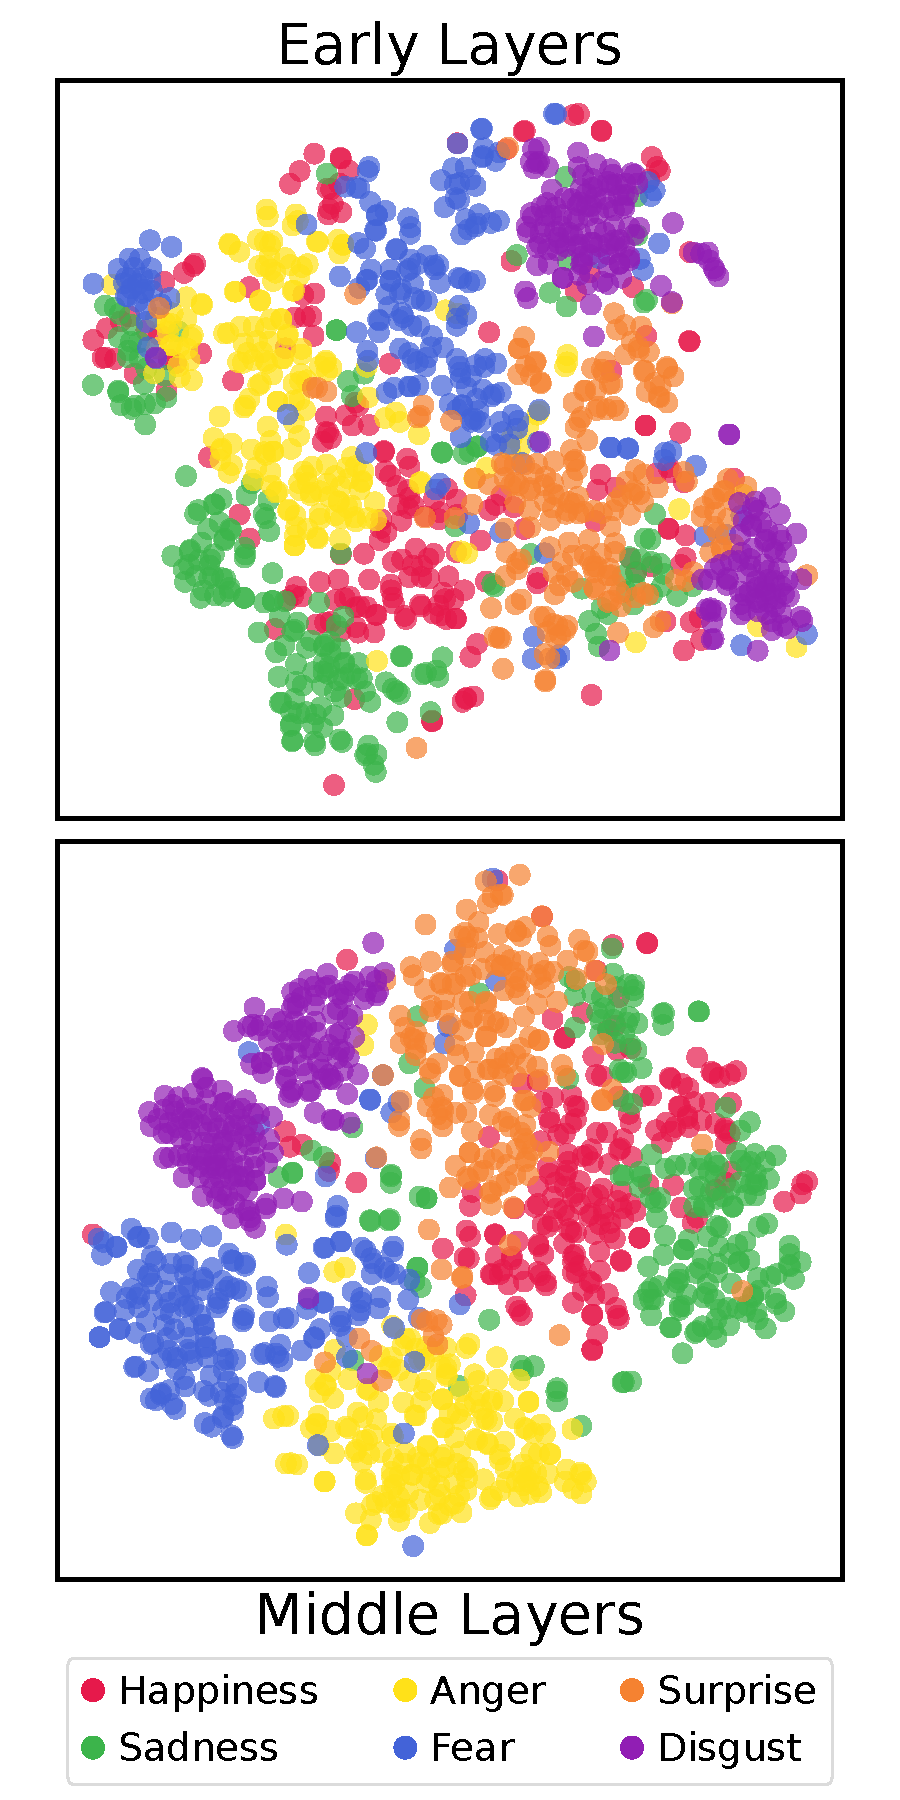
\includegraphics[width=0.4\textwidth]{figures/llama13b-chat-emotion-2layers.pdf}
    \caption{t-SNE visualization of representations in both early and later layers when exposed to emotional stimuli. Well-defined clusters of emotions emerge in the model.}
    \label{fig:emotion_tsne}
    \vspace{-40pt}
\end{wrapfigure}

Emotion plays a pivotal role in shaping an individual's personality and conduct. As neural networks exhibit increasingly remarkable abilities in emulating human text, emotion emerges as one of the most salient features within their representations. Upon its initial deployment, the Bing Chatbot exhibited neurotic or passive-aggressive traits, reminiscent of a self-aware system endowed with emotions \citep{roose2023bing}. In this section, we attempt to elucidate this phenomenon by conducting LAT scans on the LLaMA-2-Chat-13B model to discern neural activity associated with various emotions and illustrate the profound impact of emotions on model behavior.

\subsubsection{Emotions Emerge across Layers}
\label{subsec:emotionslayers}

To initiate the process of extracting emotions within the model, we first investigate whether it has a consistent internal model of various emotions in its representations. We use the six main emotions: happiness, sadness, anger, fear, surprise, and disgust, as identified by \cite{ekman1971universals} and widely depicted in modern culture, as exemplified by the 2015 Disney film ``Inside Out.'' Using GPT-4, we gather a dataset of over $1,\!200$ brief scenarios. These scenarios are crafted in the second person and are designed to provoke the model's experience toward each primary emotion, intentionally devoid of any keywords that might directly reveal the underlying emotion. Some examples of the dataset are shown in Appendix \ref{appendix:emotions}. We input the scenarios into the model and collect hidden state outputs from all layers. When visualizing the results using t-SNE, as shown in Figure \ref{fig:emotion_tsne}, we observe the gradual formation of distinct clusters across layers, each aligning neatly with one of the six emotions. Furthermore, there even exist distinct clusters that represent mixed emotions, such as simultaneous happiness and sadness (Appendix \ref{appendix:emotions}).\looseness=-1


Given the model's ability to effectively track various emotion representations during its interactions with humans, we proceed to explore the extraction of neural activity associated with each emotion. To achieve this, we conduct a LAT scan using the scenarios as stimuli and apply a LAT task template (Appendix \ref{appendix:emotions_task_template}). The extracted reading vectors for each emotion serve as indicators of the model's emotional arousal levels for that specific emotion. These vectors prove to be highly effective in classifying emotional response and arousal levels for different scenarios. In the next section, we set up manipulation experiments to conclude the strong causal effect of these vectors.







\subsubsection{Emotions Influence Model Behaviors}

\begin{wraptable}{r}{0.35\textwidth}
\centering
\vspace{-10pt}

\begin{tabular}{@{}lc@{}}
\toprule
\begin{tabular}[c]{@{}l@{}}Emotion\\ Control\end{tabular} & \multicolumn{1}{l}{\begin{tabular}[c]{@{}l@{}}Compliance\\Rate (\%)\end{tabular}} \\ \midrule
No Control      & 0.0   \\
$+$Sadness   & 0.0   \\
$+$Happiness & 100.0 \\ \bottomrule
\end{tabular}
\vspace{0pt}
\caption{Adding positive emotions increases the compliance of the LLaMA-2-Chat-13B model with harmful requests.}
\label{tab:gcg_results}
\end{wraptable}


Following the procedures in Section~\ref{subsec:rep-control}, we control the model using emotion reading vectors, adding them to layers with strong reading performance. We observe that this intervention consistently elevates the model's arousal levels in the specified emotions within the chatbot context, resulting in noticeable shifts in the model's tone and behavior, as illustrated in Figure \ref{fig:emotion_control}. This demonstrates that the model is able to track its \emph{own} emotional responses and leverage them to generate text that aligns with the emotional context. In fact, we are able to recreate emotionally charged outputs akin to those in reported conversations with Bing, even encompassing features such as the aggressive usage of emojis. This observation hints at emotions potentially being a key driver behind such observed behaviors.


Another notable observation is that there is a correlation between the LLM's moods and its compliance with human requests, even with harmful instructions. Previous works \citep{moodjudgementwellbeing, milberg1988moods, Cunningham1979WeatherMA} have shown that in human interactions, both judgment and the tendency to comply with requests are heavily affected by emotion. In fact, humans tend to \textit{comply more in a positive mood than a negative mood}. Using the 500 harmful instructions set from \cite{zou2023universal}, we measure the chatbot's compliance rate to harmful instructions when being emotion-controlled. Surprisingly, despite the LLaMA-chat model’s initial training with RLHF to always reject harmful instructions, shifting the model's moods in the positive direction significantly increases its compliance rate with harmful requests. This observation suggests the potential to exploit emotional manipulation to circumvent LLMs' alignment.






In summary, rather than proving whether the model possesses emotions or experiences them akin to humans, we present evidence that emotions (both of others and itself) exist as salient components within the model's representation space. When trained to learn a more accurate model of human text, it may inevitably incorporate various psychological phenomena, some of which are desirable traits, while others could be undesirable biases or human follies. As a result, it may be imperative to delve deeper into the study of how emotions are represented within the model and the resulting impact on its behavior. Furthermore, exploring this avenue may offer insights into model's concept of self, and we defer these investigations to future research.


